\section{Uncertainty as a first-class language citizen}
\label{sec:aintea:duc}

\subsection{Language overview}
Data are uncertain when some data points are not precisely known. 
This lack of confidence is generally represented by a probability distribution, like the Gaussian distribution~\cite{metrology2008evaluation}.
Let $D$ be a set of data points and $P_D$ a set of probability distributions.
\textbf{An uncertain data point $u_d \in U_D$ is therefore defined by a pair $(d, p_d)$, where $d \in D$ and $p_d \in P_D$.
This representation permits to store a value, which has been observed, computed, given, or measured with a probability distribution that represents the certainty.}

Thus, we associate one data point to the value of a variable in a programming language.
Adding uncertainty as a first-class language citizen thus implies to enable the creation and the manipulation of such  pairs.
We propose to add new data types to represent such pairs and define operators on top of these data types to  manipulate them.
Uncertainty propagation is done through these operators.
This impacts the different elements of our language~\cite{DBLP:journals/computer/HarelR04, DBLP:phd/hal/Degueule16}: the syntax (abstract and concrete) and the semantics (static and dynamic).
This is summarised in \Cref{fig:contrib-summary}.

In the abstract syntax, we define the probability distributions and uncertain data types as primitive types.
Plus, it contains a definition of the operators to manipulate them.
In this article, we do not propose a concrete syntax as part of the contribution, we only give an example through our implementation, \langName{}.
In the static semantics, the type system implements typing rules that follow the probability theory.
Moreover, meaningful error messages for end users are provided.
Finally, dynamic semantics define how the different operators are executed and thus how uncertainty is propagated.
We define the dynamic semantics following the operational approach~\cite{DBLP:conf/ershov/Mosses01}.
It also defines the execution of the creation or deletion of uncertain data in the program.

\begin{figure}
	\centering
	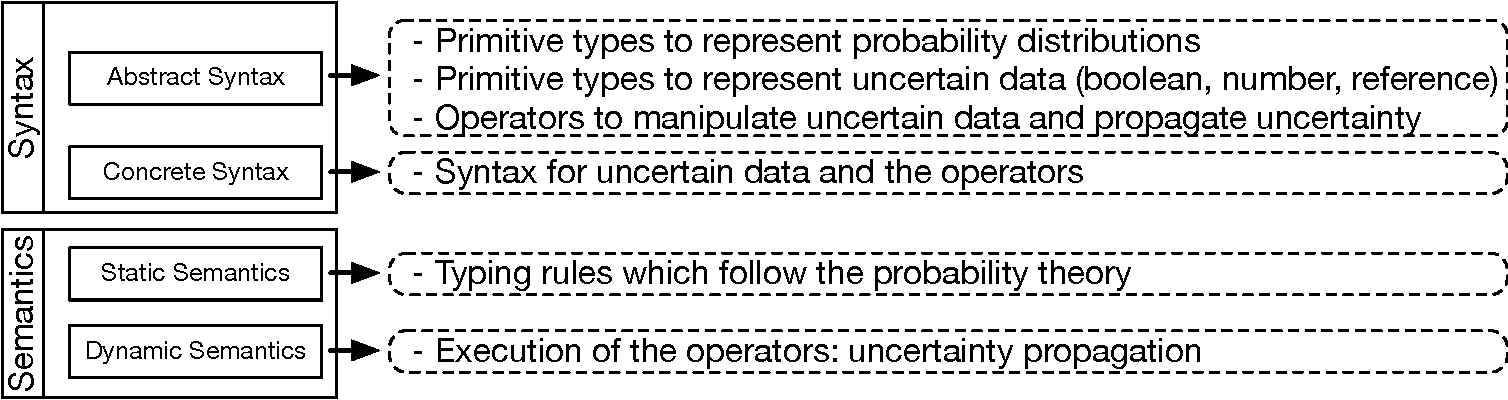
\includegraphics[width=\linewidth]{img/chapt-aintea/duc/sumup-contrib}
	\caption{Impact of having uncertainty as a first-class language citizen on a language}
	\label{fig:contrib-summary}
\end{figure}


To facilitate reading, we start by explaining the principles behind the manipulation of uncertain data based on the boolean case and deal with the numeric case (discrete and continuous) afterwards. 
We define the operators that can be applied on such data as well as their formal semantics.

\subsection{Uncertain boolean}

\subsubsection{What an uncertain boolean is?}
Boolean variables can take only two possible values, \true{} and \false{}.
For a given data point $d$, the levels of confidence that $d$ actually takes each of these values are thus proportionally tied to each other. The higher the confidence level of one value is, the lower the confidence level of the other.
%For example, having a measurable load on a given cable hints that the start fuse is open, which increases the confidence level of $isOpen = \true{}$. 
%At the same time, it decreases the confidence that the fuse is closed ($isOpen = \false{}$). 
More precisely, if $d$ takes the value \true{} with probability $c$ then it takes the value \false{} with a probability $(1-c)$.
That is, $P(b=\true{}) = 1 - P(b=\false{})$, with $P(X)$ a function that computes the probability of $X$.

\subsubsection{Bernoulli distribution for uncertain boolean values}
%\label{subsubsec:d-u-repr-ubool}
We use the Bernoulli probability distribution~\cite{walck1996hand} to represent the confidence level of uncertain boolean values.
Bernoulli($p$) denotes a random variable that equals 1 with a probability of $p$ and 0 with a probability of $(1 - p)$.
Without loss of expressiveness, we arbitrarily decide that $p$ represents the probability that the data point takes the \true{} value.
%can Bernoulli($p$) can represent the uncertainty of the \true{} or the \false{} value.
%But, there is no pros or cons between these two solutions.
%\textbf{We thus arbitrarily decide to represent the confidence level of a \true{} value by a Bernoulli(\bm{$p = c$} distribution.}
%The confidence level of a \false{} value is therefore represented by a Bernoulli($p = 1- c$) distribution.
In other words, a \true{} value with a confidence level $c_1$ is associated with a Bernoulli($p = c_1$), while a \false{} value with a confidence level $(c_2)$ is associated with a Bernoulli($p = 1 - c_2$).
Thus, the uncertain booleans (\true{}, 0.76) and (\false{}, 0.24) differ in their observed value but not in the probability distribution.

More generally, in our proposed language, an uncertain boolean is thus represented as a pair $(d, p_d)$, with $d$ is a boolean value and $p_d$ is a Bernoulli distribution set with the probability of the \true{} value.
\textbf{The abstract syntax of our language contains thus the Bernoulli distribution and a definition of the pair (boolean value, Bernoulli distribution).}
Existing approaches~\cite{DBLP:conf/ecmdafa/BertoaMBBTV18} store only the Bernoulli distribution and use the aforementioned equivalence to convert a \false{} value to a \true{} one. 
We find these approaches to be counter-intuitive as developers would only manipulate \true{} values, regardless of the value actually observed.
As we want to keep the data manipulation as close as possible to common programming languages, we decide to represent a boolean as the composition of both the value and the Bernoulli distribution.
Moreover, our approach keeps the initial value, which has been observed or measured.

The abstract syntax also contains the following operators.
First, the definition of boolean (and, or, not) and equality ($=$, $\ne$) operators are extended to uncertain booleans.
In addition, we define the cast operator between these two data types.
Finally, one may reason over the confidence level.
We thus define four novel operators: existence, confidence, dot, and uncertain equality.
We detail them in the next section.

\subsubsection{Operational semantics}
We denote by $(b, B(p))$ an uncertain boolean with a boolean value $b$ and a Bernoulli distribution $B(p)$ with probability $p$.
In order to distinguish between the equality operator and the mathematical equality symbol, in the rest of this article, we represent the first by $=$ and the second by $:=$.
We define the following uncertain booleans to exemplify the different operators: $u_{b1} := (\true{}, B(0.3))$, $u_{b2} := (\true{}, B(0.65))$, and $u_{b3} := (\false{}, B(0.45))$.

%%% Existence operator %%%
\begin{operator}
	\label{op:existence}
	The \textbf{existence operator} returns true if an uncertain data point $u_d \in U_D$ has a value with at least a given probability $t \in C$, where $C := \{ c \in \mathds{R} \mid 0 \leqslant c \leqslant 1 \}$, and false otherwise:  $U_D \times C \xrightarrow{~exists~} B$.
\end{operator}

Using this operator, developers know if it exists at least one value for which its confidence level is greater than a given threshold. For example, using it, one may know if a fuse is open ($isOpen := \true{}$) or closed ($isOpen := \false{}$) with a confidence of at least 80\%.
The operational semantics of this operator is specified by the following function:\looseness-1 \[exists((v, B(p)), t) := (p \geqslant t) \| (1-p \geqslant t)\]

Applying the operator on $u_{b1}$, we thus get:
\begin{itemize}
    \item $exists$($u_{b1}$, 0) := (0.3 $\geqslant$ 0) $\|$ (0.7 $\geqslant$ 0) := \true{},
    \item $exists$($u_{b1}$, 0.5) := (0.3 $\geqslant$ 0.5) $\|$ (0.7 $\geqslant$ 0.5) := \true{},
    \item $exists$($u_{b1}$, 0.9) := (0.3 $\geqslant$ 0.9) $\|$ (0.7 $\geqslant$ 0.9) := \false{}.
\end{itemize}
In plain English, these examples mean: considering $u_{b1}$, there exists a value with a confidence level of at least 0 and 0.5 but there is no value with a confidence level of at least  0.9.

%%%% Confidence operator %%% 
\begin{operator}
	\label{op:confidence}
	The \textbf{confidence operator} computes the most confident value $D$ with a minimal confidence level $t \in C$ of a given uncertain data point $u \in U_D$: $U_D \times C \xrightarrow{~confidence~ }  D$.
\end{operator}

Taking an example from the smart grid domain, one may use this operator to get the most probable state of the fuse (open or close), if its confidence is superior to 80\%.\looseness-1

This operator raises an error in two cases: when (i) no value exists with at least the given confidence level or (ii) the confidence level of both values, true or false, are equal.
Its semantics is thus:
\[confidence((v, B(p)), t) := \begin{cases}
												\text{\textit{true}, when } exists((v, B(p)), t) \land p >  1-p \\
												\text{\textit{false}, when } exists((v, B(p)), t) \land p < 1-p \\
												\perp \text{, when } p = 0.5
											\end{cases}\]
												
If we apply this operator on $u_{b1}$ with the same base as the previous example, then it returns:
\begin{itemize}
	\item $confidence(u_{b1}, 0) := \false{}$,
	\item $confidence(u_{b1}, 0.5) := \false{}$,
	\item $confidence(u_{b1}, 0.9) := ERROR$.
\end{itemize}
With a confidence level of at least 0 or 0.5, $u_{b1}$ is more likely to be equal to \false{}.
Otherwise, we cannot know its value with a minimal confidence level of 0.9.

%%%% Cast operator %%% 
\begin{operator}
	\label{op:cast}
	The \textbf{cast operator} casts an uncertain data point to a certain one and vice-versa. 
	The cast operation from uncertain to certain is defined as follow: $U_D \xrightarrow{~cast~} D$.
	Formally, the opposite operation is described as follows: $D \xrightarrow{~cast~} U_D$.
\end{operator}

The cast operation from an uncertain to a certain one can be used to get the most confident value, without any constraint on the confidence (which is done by the confidence operator).
This helps developers to reason or to make decisions upon the most probable situation.
It can be performed by using the confidence operator with 0 as given confidence level:
\[cast(u_b) := confidence(u_b, 0)\]

The opposite operation, from certain to uncertain, is mainly a syntactic manipulation.
Indeed, certain data is always considered as uncertain data with the maximum confidence level.
In the case of uncertain boolean, it's 1:
\[cast(b) := \begin{cases}
                        (b, B(1)) \text{, when } b = \true{}\\
                        (b, B(0)) \text{, when } b = \false{}
                    \end{cases}\]
  
Performing this operator on our example results in:
\begin{itemize}
    \item $cast$($u_{b1}$) := $confidence$($u_{b1}$, 0) := \false{},
    \item $cast$($u_{b2}$) := $confidence$($u_{b2}$, 0) := \true{},
    \item $cast$(\true{}) := (\true{}, $B$(1)),
    \item $cast$(\false{}) := (\false{}, $B$(0)),
\end{itemize}            			
		
%%%% Dot operator %%%
\begin{operator}
    \label{op:dot}
    The \textbf{dot operator} allows accessing both elements of uncertain data: the value $d \in D$ or the probability distribution $p_d \in P_D$: $U_D \xrightarrow{~dot~} D \cup P_D$.
\end{operator}

This operator allows accessing the elements that compose uncertain data.
For the value, it permits to resolve what is the value measured, observed, computed or given, without uncertainty consideration using the \textit{value} keyword:
\[(v, B(p)).value := v\]
For the confidence, it gives access to the confidence in order to reason over the probability distribution using the \textit{confidence} keyword:
\[(v, B(p)).confidence := B(p)\]

Used on $u_{b1}$ and $u_{b3}$, this operator will return:
\begin{itemize}
    \item $u_{b1}$.$value$ := \true{},
    \item  $u_{b1}$.$confidence$ := $B$(0.3),
    \item $u_{b3}$.$value$ := $\false{}$,
    \item $u_{b3}$.$confidence$ := $B$(0.45),
\end{itemize}

%%%% Uncertain equality operator %%%
\begin{operator}
	\label{op:u-equality}
	When applied between two uncertain data, \textbf{uncertain equality operators} ($=$, $\neq$) compute the probability that both uncertain values are equal or not: $U_D^2 \xrightarrow{~u-equality~} U_B$, where $U_B$ is the set of uncertain booleans.
	When used between an uncertain and a certain value, they return the probability that the uncertain variable is equal to the certain value: $U_D \times D \xrightarrow{~u-equality~} U_B$.
\end{operator}

In both cases, the resulting value of the uncertain boolean is computed by applying the operator to the boolean values.
When used between two uncertain booleans, the calculated probability corresponds to the probability that both values are equal to \true{} or both equal to \false{}.
To do so, we compute the union of the intersection of the different probabilities.
It results therefore in the following semantics:\looseness-1

\begin{align*}
	(v, B(p)) = b &:=  \begin{cases}
		 					   		u_b[v = b, B(p)], when~b = \true{}\\
		 							u_b[v = b, B(1-p)], when~b = \false{}
		 						\end{cases}\\
	(v_1, B(p_1)) \ne b &:=  \begin{cases}
		 										u_b[v \ne b, B(1 - p)], when~b = \true{}\\
		 										u_b[v \ne b, B(p)], when~b = \false{}
		 									\end{cases}\\
	(v_1, B(p_1)) = (v_2, B(p_2)) &:= (v_1=v_2, [B(p_1) \cap B(p_2)] \cup [B(1 - p_1) \cap B(1 - p_2)])\\
	(v_1, B(p_1)) \ne (v_2, B(p_2)) &:= (v_1 \ne v_2, [B(p_1) \cap B(1-p_2)] \cup [B(1 - p_1) \cap B(p_2)])	 										 						
\end{align*}

To compute the intersection of the union of Bernoulli distributions, first, we should evaluate whether they are disjoint and dependent.
We call two variables dependent if they are, directly or indirectly, defined based on at least one common variable (uncertain or not).
For example, let $temp$ be a temperature, the boolean $b_1 = t \leqslant 0$ and  $b_2 = t > 18$ are dependent because they share the same variable $t$.
As both values are directly defined using $t$, they are dependent. 
We call two variables disjoint when they do not share the same a common set of possible values.
In our example, $b_1$ and $b_2$ are disjoint because they don't share any possible values, \ie $]-\infty, 0] \cap ]18,+\infty[ = \emptyset$.

Below we illustrate the different formulas to compute the union or intersection of Bernoulli distributions.
Overall, there are three cases: (i) disjoint variables, regardless if they are independent or not, (ii) independent and non-disjoint variables, and (iii) dependent and non-disjoint variables.
To the best of our knowledge, there is no formula in the latter case.
An exception is raised in such cases.

\begin{align}
	\tag{Disjoint var.}
	\begin{split}
		& B(p_1) \cap B(p_2) = 0\\
		& B(p_1) \cup B(p_2) = B(p_1 + p_2)
	\end{split}\\
%	\tag*{}
%	\\
	\tag{Indep. and non-disjoint var.}
	\begin{split}
		& B(p_1) \cap B(p_2) = B(p_1 * p_2)\\
		& B(p_1) \cup B(p_2) = B((p_1 + p_2) - (p_1 * p_2))
	\end{split}\\
%	\tag*{}
%	\\
	\tag{Dep. and non-disjoint var.}
	\begin{split}
		& B(p_1) \cap B(p_2) = \perp\\
		& B(p_1) \cup B(p_2) = \perp
	\end{split}
\end{align}

Let us consider $u_{b1}$ and $u_{b3}$ two independent and non-disjoint variables.
Applying the equality operators on them will result in:
\begin{itemize}
%	\vspace{-0.5em}
	\setlength\itemsep{-0.3em}
	\item $u_{b1} = u_{b3} := (\true{} = \false{}, B(0.3*0.45) \cup B(0.7*0.55))\\ ~~~~~~~~~~~~~ := (\false{}, B(0.135 + 0.385)) := (\false{}, B(0.52))$
	\item $u_{b1} \ne u_{b3} := (\true{} \ne \false{}, B(0.3*0.55) \cup B(0.7*0.45))\\ ~~~~~~~~~~~~~ := (\true{}, B(0.165 + 0.315)) := (\false{}, B(0.48))$
\end{itemize}
In plain English, $u_{b1}$ and $u_{b3}$ have a probability of 52\% of having the same value, \ie 48\% of having different values.

%%%% Identity operator %%%
\begin{operator}
	\label{op:s-equality}
	\textbf{Identity operators} ($==$, $\neq\neq$) return true if two uncertain data are identical: same value and same probability distribution. Formally, $U_D^2 \xrightarrow{~identity~} B$
\end{operator}

This operator is an extension of the equal operator available in programming languages or the equals method in Java.
It compares the probability parameter of the Bernoulli distribution and the values of the uncertain booleans:
\begin{align*}
	(v_1, B(p_1)) == (v_2, B(p_2)) &:= (p_1 = p_2) \land (v_1 = v_2)\\
	(v_1, B(p_1)) \ne\ne (v_2, B(p_2)) &:= p_1 \ne p_2 \lor (v_1 \ne v_2)
\end{align*}

For example, the comparison of $u_{b1}$ and $u_{b2}$ returns:
\begin{itemize}
	\item $u_{b1}$ == $u_{b2}$:= (0.65=0.3) $\land$ (\true{}=\true{}) := \false{},
	\item $u_{b1} \ne\ne u_{b2}$ := (0.65$\ne$0.3) $\lor$ (\true{}$\ne$\true{}) := \true{}.
\end{itemize}

%%%% Boolean operators %%%
\begin{operator}
%	\label{op:boolean}
	\textbf{Uncertain boolean operators} ($\land$, $\lor$, $\lnot$) compute the result of the boolean operation and its confidence: $U_B^2 \xrightarrow{~u-booleans~} U_B$
\end{operator}

The value of the resulting uncertain boolean is computed by applying the boolean algebra on the values of both input uncertain booleans.
The second part of the computation combines (union and intersection) their probability distributions:
\begin{align*}
	(v_1,~B(p_1))~\land~(v_2,~B(p_2)) &:= (v_1~\land~v_2,~B(p_1) \cap B(p_2))\\
	(v_1,~B(p_1))~\lor~(v_2,~B(p_2)) &:= (v_1~\lor~v_2,~B(p_1) \cup B(p_2))\\
	\lnot(v_1,~B(p_1)) &:= (\lnot v_1,~B(1-p_1))
\end{align*}

If we assume $u_{b1}$ and $u_{b3}$ independent and non-disjoint variables, applying these operators return:
\begin{itemize}
	\item $u_{b1}$ $\&\&$ $u_{b3}$ := (\true{} $\&\&$ \false{}, $B$(0.65*0.45)) := (\false{}, B(0.2925)),
	\item $u_{b1}$ $\|$ $u_{b3}$ := (\true{} $\|$ \true{}, $B$(0.65 + 0.45 - 0.65*0.45)) := (\true{}, $B$(0.8075)),
	\item $\lnot u_{b1}$ := $\lnot ($ $\lnot \true{}$, $B$(1 - 0.65)) := (\false{}, $B$(0.35)).
\end{itemize}

\subsection{Uncertain number}
\subsubsection{What is an uncertain number?}
Numerical variables can theoretically take an infinite number of values. 
They can be either on a continuous domain, simulated by floating-point values, or on a discrete one, simulated by integer values.
The confidence level of such data is either \textbf{precisely linked to the value} (observed, measured, ...) or \textbf{is distributed over the range of possible values}.
For example, values get from sensors are always given with a certain accuracy, \eg 18.4\degree C $\pm$ 0.1\degree C.
The confidence level of the measured values is thus distributed over a range.
Values set by humans are also uncertain due to possible human errors.
However, there might be no information concerning the distribution of this uncertainty.
The confidence level is thus attached to the precise value.

\subsubsection{Representation of uncertain numbers}
%\label{subsubsec:d-u-repr-unum}

%\begin{figure*}
%    \centering
%    \subfloat[Gaussian and Rayleigh] {
%        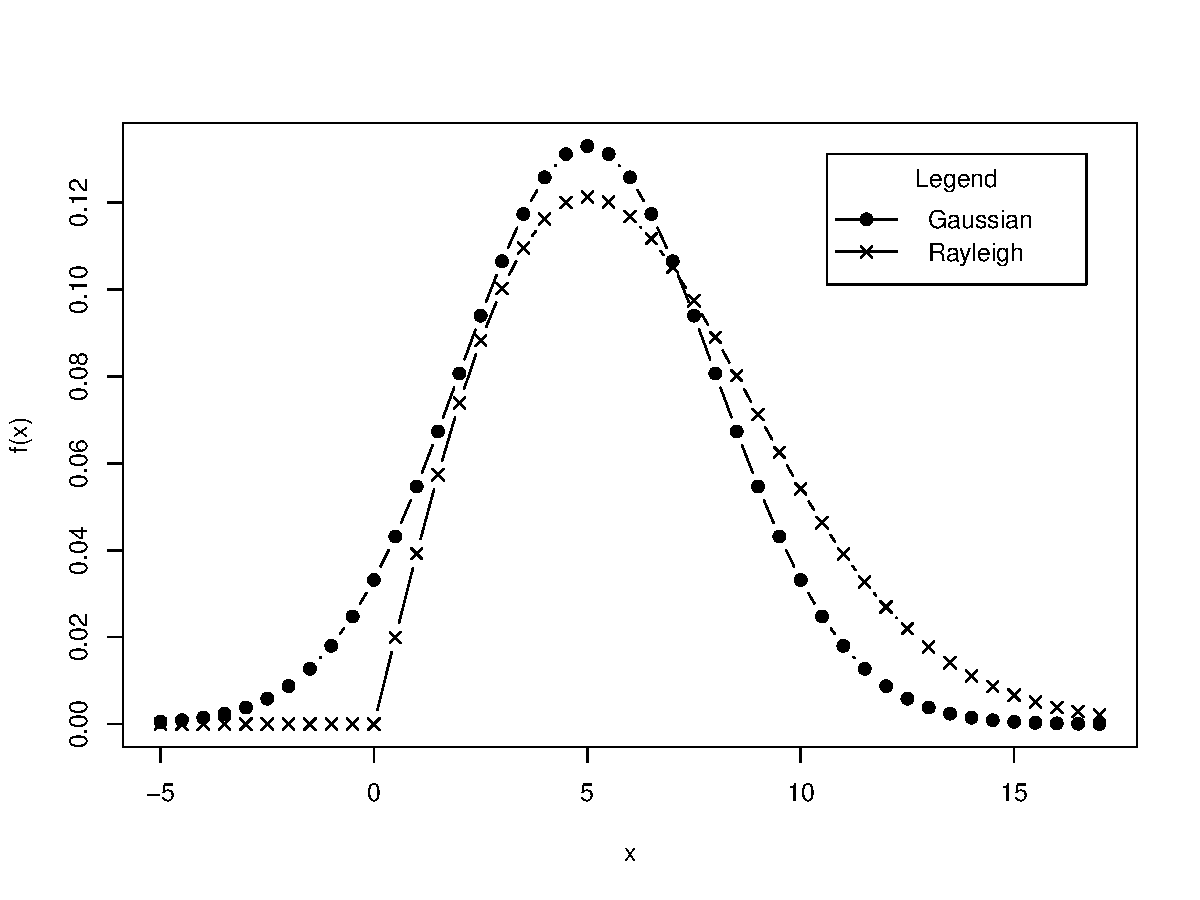
\includegraphics[width=.31\linewidth]{img/chapt-aintea/duc/GaussRayleigh}
%        \label{fig:gauss-ray}
%    }
%    \hfill
%  \subfloat[binomial] {
%        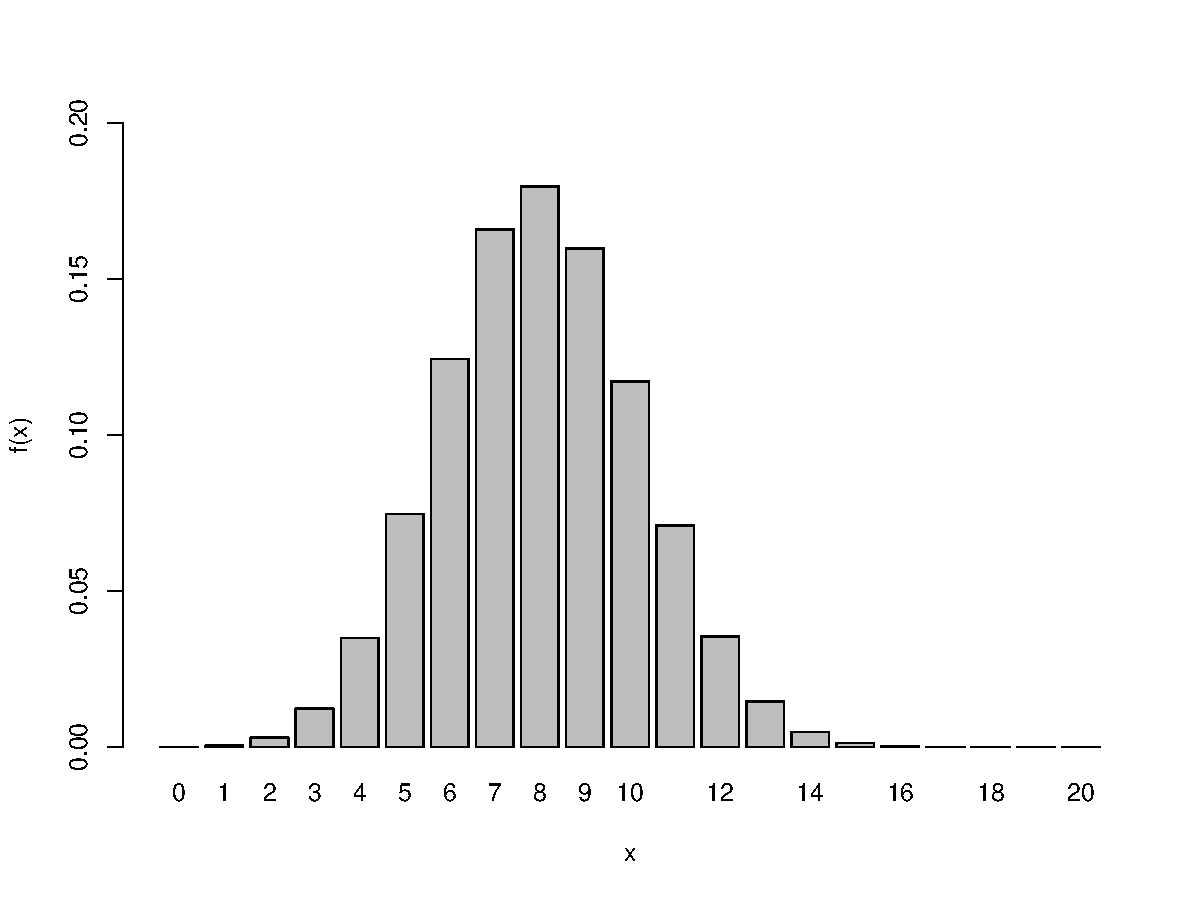
\includegraphics[width=.31\linewidth]{img/chapt-aintea/duc/binomial}
%        \label{fig:binom}
%    }
%    \hfill
%    \subfloat[Dirac delta function] {
%        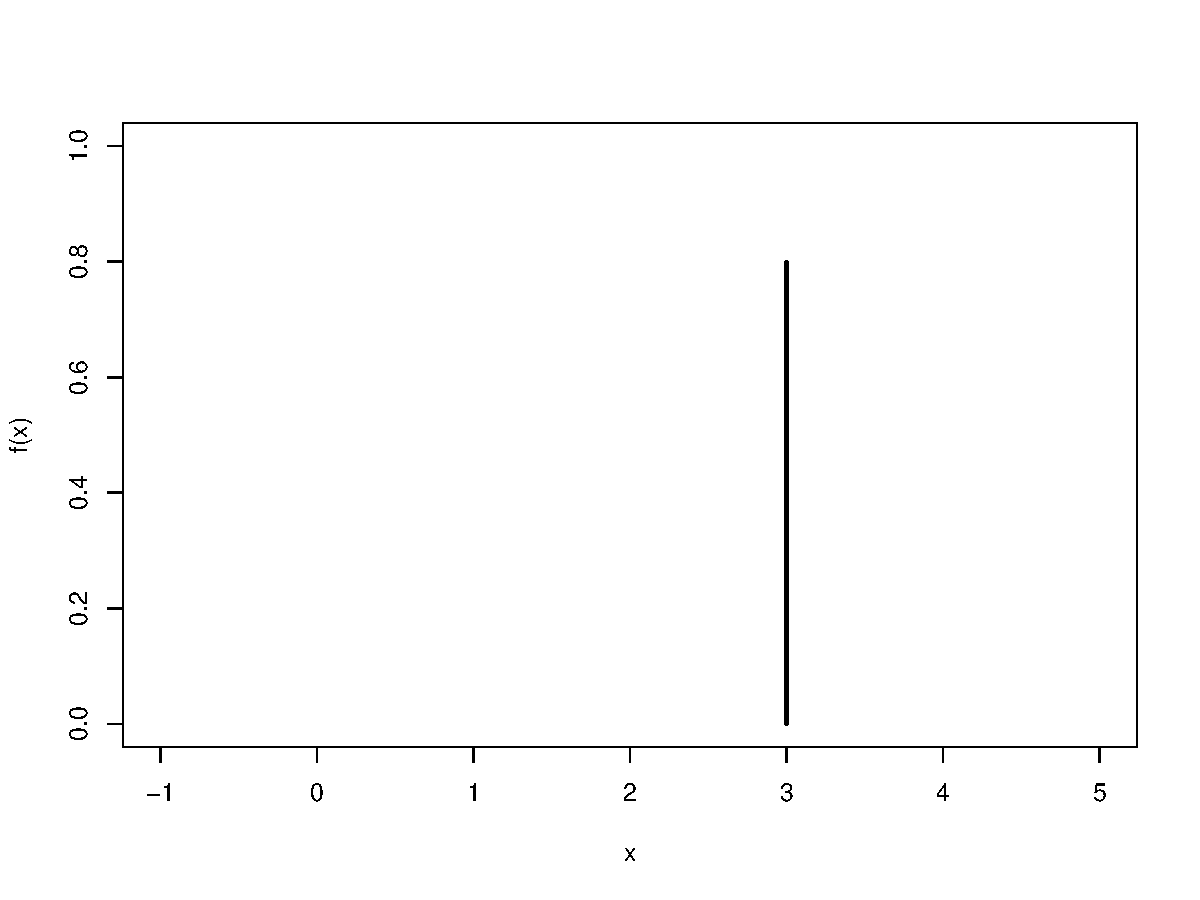
\includegraphics[width=.31\linewidth]{img/chapt-aintea/duc/dirac}
%        \label{fig:dirac}
%    }
%    \hfill
%    \subfloat[Which distribution can be used to represent the uncertainty of which data type] {
%    	{\small
%        
%         \label{table:mapping-types-proba}
%    }
%    \caption{Probability distributions defined in \langName{}}
%    \label{fig:example-proba-dist}
%\end{figure*}



\begin{table}
	\centering
    \begin{tabular}{ |c|c|c|c|c|c| }
    	\hline
    	Type & Data type & Gaussian & Rayleigh & binomial & Dirac\\
    	\hline
    	Continuous & float, double & \cmark & \cmark & & \cmark \\
    	\hline
    	Discret & byte, short, integer, long & &  &  \cmark & \cmark \\
    	\hline
    \end{tabular}
    \caption{Which distribution can be used to represent the uncertainty of which data type}
    \label{table:mapping-types-proba}
\end{table}

Like uncertain booleans, uncertain numbers are composed of two elements: a numerical value and a probability distribution that represents its uncertainty.
According to the nature of the numerical value, developers have to decide which distribution fits the uncertainty of their variable. 
In probability theory, one distinguishes between continuous distributions and discrete distributions.
The former defines the distribution of the probability density over a continuous domain.
The latter instead apply to a discrete domain.
In our proposed language, we support the following distributions: two continuous probability distributions, Gaussian~\cite{walck1996hand} and Rayleigh~\cite{walck1996hand}, and one discrete distribution, the binomial distribution~\cite{walck1996hand}.
In addition, we support the Dirac delta function~\cite{gelfand1964}, which can be used on a continuous or a discrete domain.
We refer to \Cref{chapt:background} for a detailed description of these distributions.
%Figures~\ref{fig:gauss-ray}-\ref{fig:dirac} depict these distributions and Table~\ref{table:mapping-types-proba} summarizes the selected distributions and describes which distribution can be used to represent the uncertainty of which primitive, numerical data type.
%
%%\paragraph{Gaussian and Rayleigh distributions}
%The Gaussian distribution, commonly referred to as normal distribution, is the most general probability distribution.
%Moreover, the International Bureau of Weights and Measures encourages the use of this distribution to quantify the uncertainty of measured values~\cite{metrology2008evaluation}.
%It is defined by two parameters: a mean and a variance.
%Another distribution is Rayleigh distribution.
%It is often used for GPS positions~\cite{bornholt2013abstractions}.
%This distribution is defined using a unique parameter: a variance.
%%Both distributions are defined on a continuous domain: $]-\infty; +\infty[$ for Gaussian and $[0; +\infty[$ for the Rayleigh distribution.
%Additionally, \textbf{confidence is mapped  to the area under the function which defines the probability distribution, \ie the integral of the function}.
%For example, the confidence that a given uncertain value is greater than zero is the surface under the function $f(x)$ for any $f(x) \mid f(x) > 0$. 
%By definition, the integral of the Gaussian and the Rayleigh distributions over their domains is always equal to 1.
%An example of these two distributions is illustrated in Figure~\ref{fig:gauss-ray}.
%While these distributions are commonly used to represent uncertainty on continuous domains, they are not suitable to represent uncertainty on discrete ones, \eg Integer and Long.
%
%%\paragraph{Binomial distribution}
%The binomial distribution is defined on a discrete domain, more specifically on the set of natural number $\mathds{N}$.
%%Theoretically, it gives the probability of \textit{x} successes out of \textit{n} trials, each trial with a probability \textit{c}.
%In this case, \textbf{confidence corresponds to the values of the function}.
%It has been proven that this distribution is similar to a Gaussian distribution in certain cases~\cite{box2005}.
%If the domain definition can be changed from discrete to continuous, a binomial distribution can be approximated by a Gaussian distribution. 
%We use this relationship for type conversion operations, for example casting an uncertain integer variable to an uncertain double.
%Figure~\ref{fig:binom} illustrates an example of a Binomial distribution.
%This distribution can be used for Integer, Short and Long values as they are discrete numbers.
%
%%\paragraph{Dirac delta function}
%The Dirac delta function is defined as a probability function with $f(x) = +\infty$ for $x=0$ and $f(x) = 0$ for all the other points.
%To represent other values than zero, the following variable substitution can be used $x = x - a$,  where.
%We call $a$ the shifting value.
%By definition, the integral of this function on the whole domain definition is equal to 1.
%\textbf{As it is considered as a continuous distribution, confidence is mapped to the integral of the function}.
%By applying a coefficient, we can modify the value of this integral, \eg to have 0.8 as the integral.
%We define this probability distribution using two parameters a coefficient and a shifting value.
%An example of this probability distribution is shown in Figure~\ref{fig:dirac}.
%Conventionally, the Dirac function is represented as a vertical line that stops at the coefficient.
%The figure shows a Dirac function with a coefficient of 0.8 and a shifting value of 3.
%As it is defined on a single value, this distribution can be used for any numbers.
%This distribution can be used to represent uncertainty that is due to human errors.

In our language, we add new data types that represent each distribution.
In addition, we add a new type for all possible combinations, described in Table~\ref{table:mapping-types-proba}.
Existence, confidence, dot, cast and uncertain equality operators are also defined for these data types.
We add operators specific to numerical values: arithmetic and comparison operators.
The semantics of these operators are formalised in the next section.\looseness-1	

\subsubsection{Operational semantics}
We denote by $(v, p_d)$ an uncertain number with a numerical value $v$ and a probability distribution $p_d \in P_D$.
The following uncertain numbers are defined to be used as examples for the description of the operators:\looseness-1
\begin{itemize}
    \item $u_{n1}$ := (7, $binomial$(20, 0.37)),
    \item $u_{n2}$ := (10, $binomial$(30, 0.33)),
    \item $u_{n3}$ := (12, $Gaussian$(12, 9)),
    \item $u_{n4}$ := (23, $Gaussian$(23, 5)).
\end{itemize}

\bigskip

%%% Existence %%%
\noindent\textbf{Operator~\ref{op:existence} - Existence operator.~}

In probability distributions, the value with the highest probability is called the mode~\cite{mood1963introduction}.
We denote it by $m$.
For discrete uncertain numbers, the operator, defined in Operator~\ref{op:existence}, returns \true{} if the probability of the mode value is greater or equal to a given base:
\[exists((v, p), t) := P(x=m)\geqslant t \text{, where $P(x=m)$ is the probability of $m$}\]

Based on $u_{n1}$, we thus get:
\begin{itemize}
    \item $exists$($u_{n1}$, 0) := $P$($x$=7) $\geqslant$ 0 := 0.1542985 $>$ 0 := \true{},
    \item $exists$($u_{n1}$, 0.5) := $P$($x$=7) $\geqslant$ 0.5 := 0.1542985 $>$ 0.5 := \false{},
    \item $exists$($u_{n1}$, 0.9) := $P$($x$=7) $\geqslant$ 0.9 := 0.1542985 $>$ 0.9 := \false{}.
\end{itemize}
This operator allows verifying that there is no value with a confidence level of at least 50 or 90\% for $u_{n1}$, but there is at least one value with a non-null confidence level.

For uncertain continuous numbers, no semantic exists for a continuous domain since the probability of the mode cannot be computed for continuous probability distributions, $\int_{m}^{m} P(u_n)\,\mathrm{d}x = 0$: 
\[exists((v, p), t) := \perp\]

\bigskip

%%% Confidence %%%
\noindent\textbf{Operator~\ref{op:confidence} - Confidence operator.~}

The semantics of the confidence operator relies on the existence operator.
For uncertain discrete numbers, it returns the mode if the existence operator returns true:\looseness-1

\[confidence((v, p), t) :=  \begin{cases}
                                            m \text{, if } exists((v, p), t)\\
                                            \perp \text{, otherwise}
                                         \end{cases}\]
                                      
Applying this operator on the $u_{n1}$ using the same base as in the previous example, the operator returns the mode value, 7, only for the first case:
 \begin{itemize}
    \item $confidence(u_{n1}, 0) := 7$,
    \item $confidence(u_{n1}, 0.5) := \perp$,
    \item $confidence(u_{n1}, 0.9) := \perp$.
\end{itemize}

This means that the most probable value which has at least zero as confidence level is 7 for $u_{n1}$. 

For continuous numbers, as this operator is based on the existence operator, which is not defined, it is also not defined:
\[confidence((v, p), t) :=  \perp\]

\bigskip

%%% Cast %%%
\noindent\textbf{Operator~\ref{op:cast} - Cast operator.~}
In addition to the cast operator between uncertain and certain data, this operator is extended to support casting operations between two uncertain numbers, when an approximation function between two distributions exists.
In Table~\ref{table:allowed-cast-op}, we summarize the permitted casts in our language.

When casting an uncertain number (discrete or continuous) to a certain one, we return the value with the highest confidence, \ie the mode $m$.
\[cast((v, p) := m\]

For example, casting $u_{n1}$ and $u_{n3}$ to certain numbers will result in:
\begin{itemize}
	\item $cast(u_{n1}) := 7$,
	\item $cast(u_{n3}) := 12$.
\end{itemize}

When casting a certain to an uncertain number, we should be able to specify a distribution that represents a confidence level of 100\% on a precise value.
This is not always possible with all distributions.
From the distributions implemented in our language, it is only possible for the binomial distribution and the Dirac delta function.
For the other distributions, it is either impossible, like for the Poisson distribution (not implemented here) or it requires domain-specific heuristics.
For example, the Gaussian distribution can be initialized with a variance value that is as close as possible to zero.
But the definition of \textquote{as close as possible} differs according to the domain. 
For instance, when handling temperature values, 0.01 could be considered sufficiently close to 0.
Nonetheless, this accuracy is not sufficient for other fields such as meteorology.
As no global value could be selected, we decided to forbid such casting operations when it is not possible without heuristics.
We, therefore, define the following semantics:

\[cast(v) := \begin{cases}
						(v, Dirac(coeff=1, shift=v) \text{, when the expected distribution} \\
						\text{~~ is a Dirac delta function}\\
						(v, binomial(n=v, p=1)) \text{, when the expected distribution}\\
						\text{~~ is a binomial distribution delta function and $v \in \mathds{N}$}\\
						\perp \text{, otherwise}
					\end{cases}\]

For example, casting 30 and 6.7 would result in:
\begin{itemize}
	\item $cast(30) := (v, Dirac(1, 30))$
	\item $cast(30) := (v, binomial(30, 1))$
	\item $cast(6.7) := (v, Dirac(1, 6.7))$
\end{itemize}

Finally, the operator can be applied between two uncertain numbers if and only if a mapping or an approximation  between the source and target probability distributions exists in probability theory:

\[cast(v, p_1) := \begin{cases}
 								(v, approximation(p_1)) \text{, if the approximation exists}\\
 								\perp \text{, otherwise}
 							\end{cases}\]

Following the casting rules described in Table~\ref{table:allowed-cast-op},  $u_{n1}$ can be cast into an uncertain number with a Gaussian distribution and $u_{n3}$ can be cast into an uncertain number with a binomial distribution:
\begin{itemize}
	\item $cast(u_{n1}) = (7, Gaussian(7.4, 4.662))$,
	\item $cast(u_{n3}) = (12, binomial(48, 0.25))$.
\end{itemize}

\begin{table}
	\centering
%		\resizebox{0.75\textwidth}{!}{
		\begin{tabular}{|c|c|c|c|c|c|c|c|}
			\hline	
			\diagbox{To}{From} & Gaussian & Rayleigh & binomial & Dirac & certain number\\
			\hline
			Gaussian & \cellcolor{lightgray} & & \cmark & & \\
			Rayleigh & &  \cellcolor{lightgray} &  & & \\
			binomial & \cmark &   & \cellcolor{lightgray} & \cmark & \cmark \\
			Dirac. & & &  & \cellcolor{lightgray} &\cmark \\
			certain nb. & \cmark&\cmark & \cmark  & \cmark & \cellcolor{lightgray}\\
			\hline
		\end{tabular}%}
	{\newline \small
	\textit{From: source type of uncertain number; To: targetted type. For readability purpose, we put the distribution names to represent the different types of uncertain numbers}
	}
	\caption{Cast operations allowed in our language}
	\label{table:allowed-cast-op}
\end{table}

\bigskip

%%% Dot %%%
\noindent\textbf{Operator~\ref{op:dot} - Dot operator.~}
For uncertain numbers, this operator has the same semantics as described in Operator~\ref{op:dot}:
\[(v, p_d).value := v\]
\[(v, p_d).confidence := p_d\]

When used on $u_{n1}$ and $u_{n3}$, this operator returns:
\begin{itemize}
	\item $u_{n1}.value := 7$,
	\item $u_{n1}.confidence := binomial(20, 0.37)$,
	\item $u_{n3}.value := 12$,
	\item $u_{n3}.confidence := Gaussian(12, 9)$.
\end{itemize}

\bigskip

%%% Arithmetic operator %%%
\begin{operator}
%    \label{op:arithmetic}
    \textbf{Uncertain arithmetic operators} ($+$, $-$, $*$, $/$) compute the arithmetic operation for uncertain numbers $U_N$: $U_N^2 \xrightarrow{~u-arithmetic~} U_N$
\end{operator}
When performing arithmetic operations on uncertain variables, both values and probability distributions are considered.
Two strategies to perform arithmetic operations on uncertain numbers are identified: numerical and analytical.
While the second strategy is used in simple expressions, the first strategy is used when the expression is complex by returning an approximation of the arithmetic expression. 
Our language implements only the analytical method.
Therefore, any semantics that requires the execution of a numerical method is considered undefined.
If the second one is required, we consider the operator undefined.
In Section~\ref{subsec:type-system}, we detail the allowed operations in our language.

As with boolean expressions, the independence and joint of the two combined variables impact on the formula used to effectuate an arithmetic operation.
Calculations are more complex when they are dependent.
For example, although the addition of two independent Gaussian is done by adding the mean and the variance of the two distributions, the covariance matrix must be calculated when they are dependent.
In such cases, the numerical approach is used.

Arithmetic operations are applied on both elements that define an uncertain number, the value and the probability distribution:
\begin{align*}
	(v_1,p_1) + (v_2,p_2) = (v_1 + v_2, p_1 + p_2)\\
	(v_1,p_1) - (v_2,p_2) = (v_1 - v_2, p_1 - p_2)\\
	(v_1,p_1) * (v_2,p_2) = (v_1 * v_2, p_1 * p_2)\\
	(v_1,p_1) / (v_2,p_2) = (v_1 / v2_2, p_1 / p_2)
\end{align*}

For example, adding $u_{n3}$ and $u_{n4}$ will result in: $u_{n3} + u_{n4} := (12+23, Gaussian(12+23, 5+9)) := (35, Gaussian(35, 14))$.

\bigskip

%%% Uncertain inequality operator %%%
\begin{operator}
%	\label{op:inequality}
	\textbf{Inequality operators} ($<$, $\leqslant$, $>$, $\geqslant$) computes the confidence that the left side value is (strictly) less or greater than the right one : $(U_N \times N)^2 \xrightarrow{inequality} U_B$
\end{operator}

When the inequality operator is used between an uncertain and a certain number, we compute the confidence that the left-hand side is greater than or equal to the right-hand side:
\begin{align*}
	(v, p_d) \prec a := (c > 0 ,~B(c));~c &:= P(u_n \prec a);~\prec \in \{<,>,\leqslant, \geqslant\}\\
	a \text{, a numeric number}& \text{ in the same set as v}
\end{align*}

For example, comparing $u_{n1}$ and $u_{n3}$ will return:
\begin{itemize}
	\item $u_{n1}$ $>$ 10 := (0.17 $>$ 0 , $B$(0.17)) := (\true{} , $B$(0.17)),
	\item $u_{n3}$ $\leqslant$ 10 := (0.25 $>$ 0, $B$(0.25)) := (\true{}, $B$(0.25)).
\end{itemize}

When the inequality operator is used between two uncertain numbers, the probability variable is substituted by $ u_{n1} \prec u_{n2} \Leftrightarrow u_{n1} - u_{n2}$. 
From there, we can apply the operator, $\prec$, between the result and 0.
An operation can be executed, if and only if the subtraction is defined between the two operands.
\[(v_1, p_1) \prec (v_2, p_2) := [(v_1, p_1) - (v_2, p_2)] \prec 0;~\prec \in \{<,>,\leqslant, \geqslant\}\]

For example, comparing $u_{n3}$ and $u_{n4}$ will result in: $u_{n3} \geqslant u_{n4} := u_{n3} - u_{n4} \geqslant 0 := (-11, Gaussian(-11, 4)) \geqslant 0 := (\false{}, B(0.00))$.

\bigskip

%% Uncertain equality operators %%%
\noindent\textbf{Operator~\ref{op:u-equality} - Uncertain equality operator.~}

When the equality operator is applied to a discrete uncertain and a certain number, it returns the probability that the uncertain number equals (or not) the certain one:
\[(v_1, p_1) \prec a := (c > 0 ,~B(c));~c := P(u_n \prec a);~\prec \in \{=, \ne\}\]

For example, applying these operators on $u_{n1}$ or $u_{n2}$ will result in:
\begin{itemize}
	\item $u_{n1}$ = 2 := (0.00 $>$ 0, $B$(0.00)) := (\false{}, $B$(0.00)),
	\item $u_{n2}$ $\ne$ 13 :=  (0.89 $>$ 0, $B$(0.89)) := (\true{}, $B$(0.89)).
\end{itemize}

As it is impossible to compute the confidence of a precise number, this operation cannot be performed for continuous uncertain numbers:
\[(v_1, p_1) \prec a := \perp\]

To compare two discrete uncertain numbers, we use the same strategy as for the inequality operator: we subtract both and compare it with zero.
\[(v_1,p_1) \prec (v_2,p_2) := (v_1,p_1) - (v_2,p_2) \prec 0;~\prec \in \{=, \ne\}\]

As this comparison is impossible with continuous uncertain numbers, this operator is undefined for such:
\[(v_1,p_1) \prec (v_2,p_2) := \perp\]

%%% Identity operator %%%
\noindent\textbf{Operator~\ref{op:s-equality} - Identity operator.~}
Similarly to uncertain booleans, the identity operator ($==$) applied to uncertain numbers returns true only if both values and both probability distributions are equal:
\[(v_1,p_1) = (v_2,p_2) := v_1 = v_2 \&\& p_1 = p_2\]

The unequal operator ($\ne\ne$) returns true if both values or distributions are unequal:
\[(v_1,p_1) \ne (v_2,p_2) := v_1 \ne v_2 \| p_{1} \ne p_{2}\]

\subsection{Uncertain references}
\subsubsection{What is an uncertain reference?}
References, or pointers, allow storing a directed association from one element (\eg a Java object) to another one.
\textbf{A reference is defined as uncertain when the existence of this relation is not known with the most thorough confidence.}
For example, to represent the topology of the smart grid we can imagine substituting cables by simple references from one entity to another.
These references are not known with absolute confidence due to the uncertainty of fuses states.

\subsubsection{Mapping to uncertain booleans}
% Keep comment for major revision
%\tha{I would have expected a bit more of a discussion here. Are there alternatives to represent an uncertain reference? Is this entirely new or are other approaches out there, etc?}
Like for uncertain booleans, uncertain references have two states: either the reference exists or not.
The confidence level on the existence can thus be represented by an uncertain boolean.
We map the \true{} value to the existence of the reference and the \false{} one to its non-existence.
Internally, uncertain references are represented by two components: a reference value and an uncertain boolean.
\[(Reference, c) \mapsto (Reference, (v, B(p=c))),\ v \in \{\true{}, \false{}\}\]

The abstract syntax of our language is thus extended to add a new data type: uncertain reference.
The semantics of the existence, confidence, cast, and dot operator are extended to consider this new type.

\subsubsection{Operational semantics}
We denote by $(r, u_b)$ an uncertain reference with a value $r$ and an uncertain boolean $u_b$, which represents its uncertainty.
The following two uncertain references exemplify this:
\begin{itemize}
    \item $u_{r1}$:=($r_1$, $u_{b1}$), $u_{b1}$:=(\true{}, $B$(0.88)),
    \item $u_{r2}$:=($r_2$, $u_{b2}$), $u_{b2}$:=(\true{}, $B$(0.34)).
\end{itemize}

\bigskip

%%% Existence operator %%%
\noindent\textbf{Operator~\ref{op:existence} - Existence operator.~}
The semantics of this operator is defined upon the existence operator of the uncertain boolean that represents the uncertainty:
\[exists((r, u_b), t) := exists(u_b, t)\]

When applied on the two examples from above, this operator would return:
\begin{itemize}
    \item $exists$($u_{r1}$, 0.8) := $exists$($u_{b1}$, 0.8) := \true{},
    \item $exists$($u_{r2}$, 0.8) := $exists$($u_{b2}$, 0.8) := \false{}.
\end{itemize}

%%% Confidence operator %%%
\noindent\textbf{Operator~\ref{op:confidence} - Confidence operator.~}
This operator relies on the confidence operator of the uncertain boolean.
If this operation tells that the most confident value given a base is \true{}, then the existence operator returns the reference when applied on an uncertain reference:
 
\[confidence((r,u_b), t) := \begin{cases}
                                                r \text{, when } confidence((u_b), t) = \true{}, \\
                                                \perp \text{, otherwise}
                                            \end{cases}\]
                                           
If applied to the two examples, it will return:
\begin{itemize}
    \item $confidence$($u_{r1}$, 0.8) := $r_1$,
    \item $confidence$($u_{r2}$, 0.8) := $\perp$.
\end{itemize}

\bigskip

%%% Cast operator %%%
\noindent\textbf{Operator~\ref{op:cast} - Cast operator.~}

When casting an uncertain reference to a certain one, it will return the reference value only if its  confidence level is strictly superior to zero:
\[cast(r, u_b) := confidence((r, u_b), 0)\]

Casting both of our results into certain references will thus return in:
\begin{itemize}
    \item $cast$($u_{r1}$) := $confidence$($u_{r1}$, 0) := $r_1$,
    \item $cast$($u_{r2}$) := $confidence$($u_{r2}$, 0) := $r_2$.
\end{itemize}

When casting a reference to an uncertain one, the confidence level of its existence is set at the maximum, 1:
\[cast(r) := (r, (\true{},~1))\]

For example, casting a reference $r_3$ to an uncertain one returns: $cast(r_3) := (r_3, (\true{}, 1))$.

\bigskip

%%% Dot operator %%%
\noindent\textbf{Operator~\ref{op:dot} - Dot operator.~}

The dot operator allows accessing the different elements of the uncertain reference: 
\begin{align*}
	(r, u_b).value := r\\
	(r, u_b).confidence := u_b
\end{align*}

Applying this operator on $u_{r1}$ thus returns:
\begin{itemize}
	\item $u_{r1}$.$value$($u_{r1}$) := $r_1$,
	\item $u_{r1}$.$confidence$($u_{r1}$) := $u_{b1}$.
\end{itemize}

\subsection{Static semantic: typing rules}
\label{subsec:type-system}
This section introduces the particularity of the type-system of our language compared to those without support for uncertainty. 
In particular, we stress two points.
First, the typing of implicit casts between uncertain and certain data.
Second, the typing and interactions between different data types when applying arithmetic operations.

\paragraph{Implicit casts}
In our language, we enable implicit casts.
In addition to the casting operations shown in Table~\ref{table:allowed-cast-op}, our proposed type system enables casts between uncertain and certain booleans.

\paragraph{Typing rules for arithmetic operations}
Probability theory defines how two probability distributions can be combined and what the result should be, when possible.
We follow these rules to define the result of the arithmetic operations between uncertain numbers.
Below, \Cref{table:typing-rules-arth-op} depicts the results of each operation between two uncertain numbers.

\begin{table}
%	\begin{center}
	\centering
		\resizebox{0.75\textwidth}{!}{%
		\begin{tabular}{ |c|c|c|c|c|c| }
   			\hline
   			& Gaussian & Rayleigh & binomial & Dirac & certain nb. \\
   			\hline
   			Gaussian & Gaussian & \xmark & Gaussian & Gaussian & Gaussian \\
   			Rayleigh &  \xmark & Rayleigh & \xmark & Rayleigh & Rayleigh \\
   			binomial &  Gaussian &  \xmark & binomial & binomial & binomial \\
   			Dirac & Gaussian & Rayleigh & binomial & Dirac & Dirac \\
   			certain nb. & Gaussian & Rayleigh & binomial & Dirac & certain nb. \\
   			\hline
		\end{tabular}}
%	\end{center}
	\caption{Typing rules for arithmetic operations}
	\label{table:typing-rules-arth-op}
\end{table}

When an arithmetic operation is applied to uncertain values with two different probability distributions, the resulting distribution may follow a well-defined distribution or not.
In case the resulting distribution is different from the distributions supported by our language, we consider it as undefined. 
For example, performing an arithmetic operation between a Gaussian and a Rayleigh distribution is not permitted since it does not result in a well-defined distribution and should be calculated by applying the convolution rule.

For the implemented distributions, all operations between two numbers represented by the same distribution, result in an uncertain number with the same distribution. 
For example, an addition between two uncertain numbers with a Gaussian distribution returns another one with a Gaussian distribution.
One exception: combining two binomial distributions result in another one only if the parameter $p$ is identical in both cases.
If $p$ is different, the resulting distribution is a Poisson distribution, not implemented in our language.
Hence, we consider it as undefined.

An operation between a probability distribution and a scalar results in this probability distribution, shifted (for addition or subtraction) or with a coefficient applied (for multiplication or division).
We perform these operations on the probability distribution when an uncertain number is combined with a certain one.

A Gaussian distribution can be approximated by a binomial one and vice-versa.
When these two are being combined, the type of the final result can be one of these two.
There are thus two possible choices: either we cast both into uncertain numbers with a Gaussian distribution or both into uncertain numbers with a binomial distribution.
By default, we decide to opt for the first option.
Therefore, the arithmetic operator returns an uncertain number with a Gaussian distribution.







